\fullwidthbox{22-7 - Setting up Camp \passage{X-Ray}}{
After about 6 hours of caving in \passage{Vrtnarija}, we finally made it down. 
We met Gergely and James on the way down just as they were exiting the cave. The last bolt on \passage{Zimmer} before camp is horrible: it needs rebolting and rerigging. 
15 cm lower would be awesome. 

We set up the tent at the camp, which required some stone movement. 
Mike got water from nearby \passage{Zimmer} and Jarv and I built up the tent, while Kate was smoking. 
NEED WEED! We should have thought about it beforehand. 
Now listening to Massive Attack and getting Raptured. Oh yeah! 

Kate is now setting up sleeping space, while Jarv is away to get more water.

Camp is slowly getting established, we're now looking forward to Worms World Party. 
Mike is cooking. 
Weed is really a missing resource. 
So far so good. 
About 5 metres from camp is a hole with audible rush of water in it. This quickly got established as peeing corner, hoping it's not a lead... 
\name{Nick}
}


\marginnote{The fast increasing smell of urea put a stop to this practice, and instead a BDH container emptied in \passage{Zimmer} was used.}




\section{The discovery of Wonderland}

\margininbox{Leopard}{
     \begin{itemize}
    \item Gergely Ambrus
    \item Andy Jurd
    \end{itemize}}{\explo}


It was another rainy day. Arriving not too long ago to the plateau, the thrill of the new possibilities for discovery was boiling in my venes[sic].
While drinking in-countably many cups of tea, we discussed the possibilities with the old lags who are always the source of infinite
wisdom. Dave suggested to check out \passage{Leopard}, the passage that
opened from \passage{Zimmer}, just opposite of \passage{Friendship Gallery}.
Martin McGowan had been there some 10 years ago, but information was
unclear, and the chances for the continuation there had been at least
dubious -- so given it is so close to camp, why not give it a go?

\margininbox{24-7 2:05pm}{
Great push down \passage{Korita} today - 8 bolts, surveying etc. It's GOING,
GOING, GOING\ldots{} Go THERE! (But try and avoid rigging future
pitches in or near the water\ldots{}) Andy and Gergely have left to
push \passage{Leopard} - James and Dan to survey \passage{Muddy Window} and then go for a
jolly below \passage{Big Rock}. \name{Tetley}}{\logbook}

Andy was sort of up to going underground, and I felt super happy to go caving with one of the heroes of the discovery of many underground passages on \passage{Migovec}. So the usual endless faffing started, packing good amounts of food, Vitaminski, gas canisters, and some Zganje, and
finally, well in the afternoon, we started our descent towards the unknown.

The way down we got again used to the feeling of hanging in big abysses on dubious bolts, which proved to be quite useful for what followed. Reaching \passage{Zimmer}, Andy chatted to Tetley and Myles (who were already at camp), while I bounced with the rope to the window and put in two bolts for having an easier start the next day. Having a sleep at camp was OK, although Andy did not seem to be very happy about the limited comfort of \passage{X-Ray}, and \bignote{he stated that he was too old for underground camping -- a fact that changed little of our plans} for the next day, of course.

So, in the morning we climbed up to the gallery, and secured the rope to a large boulder at the top of the climb. \passage{Leopard} was very nice, a typical phreatic tube, with formations resembling the spots of a leopard on its walls, and also with a fairly good draught (I am always keen on following the wind). At the other end, a dark muddy pitch-head waited us, with a good number of scary, loose boulders around it. We again noticed that \passage{Gardeners' World} is so aptly named, and
started to clean up the place. We could not remove the largest rock, tilted against the wall, so decided to go underneath it. We were not quite sure that it is going to stay, but it is still there, after
hundreds of cavers have passed beneath\ldots{}

\begin{figure*}[t!]
\checkoddpage \ifoddpage \forcerectofloat \else \forceversofloat \fi
\frame{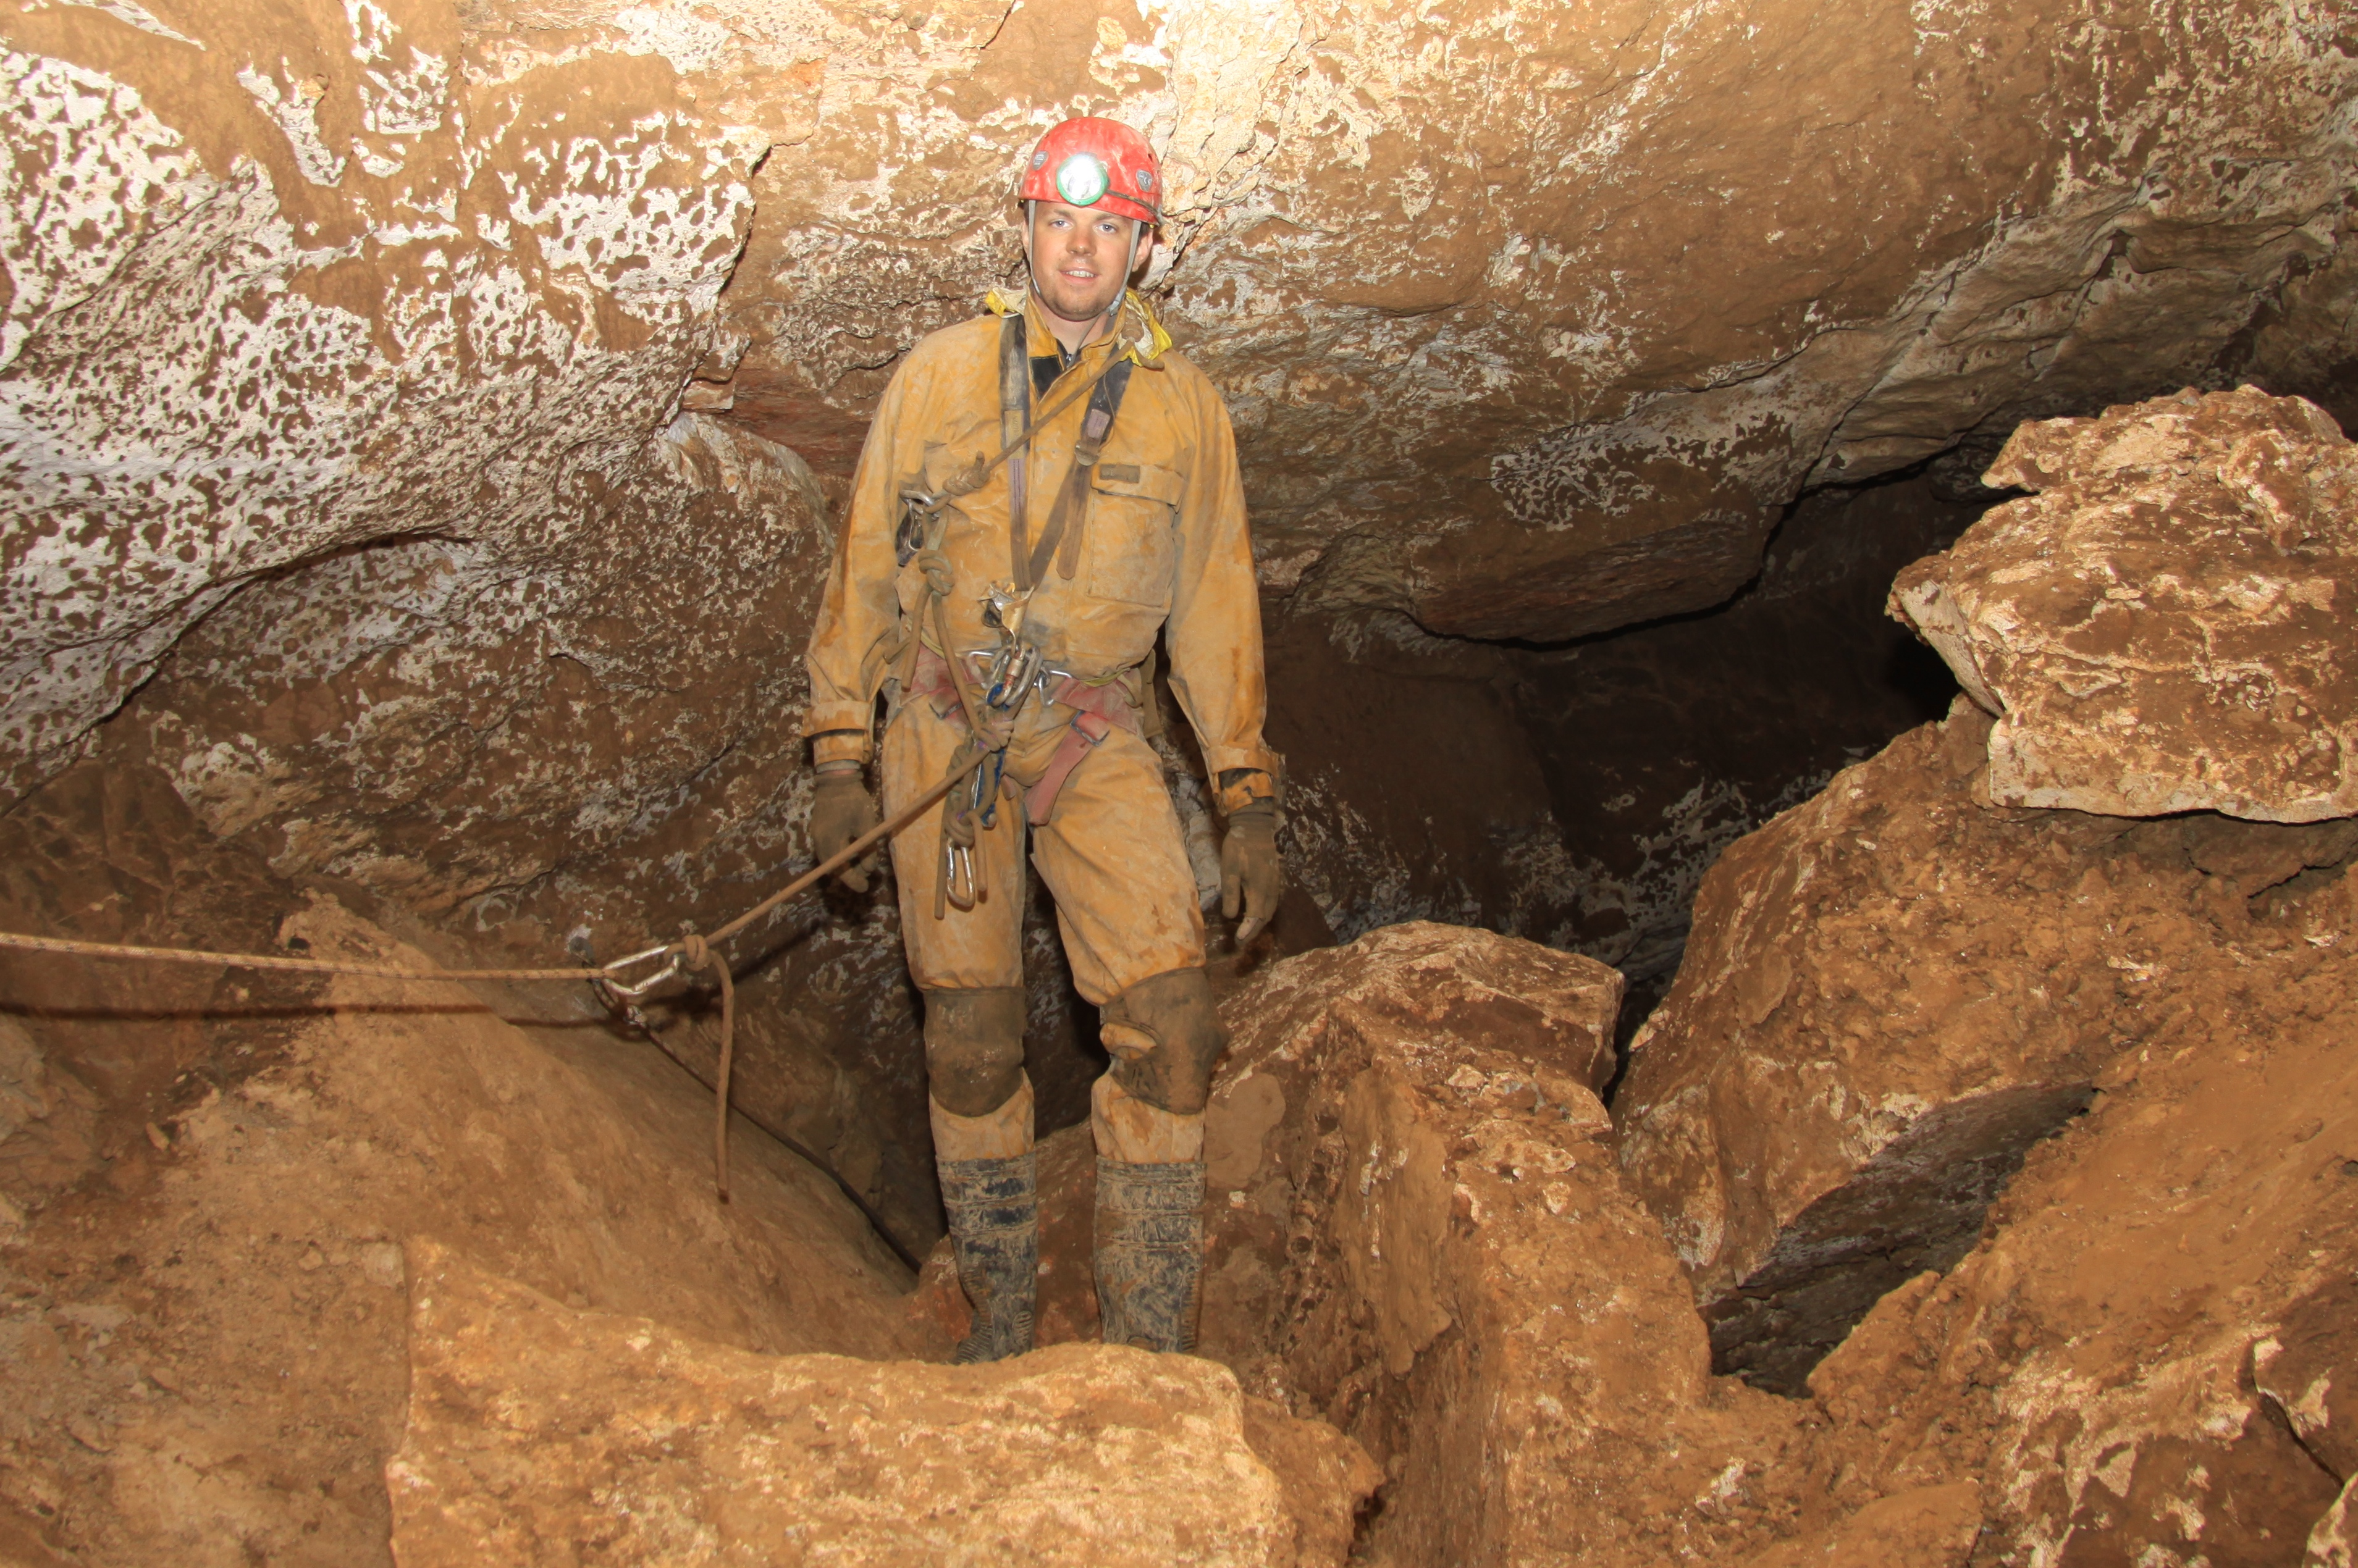
\includegraphics[width=\linewidth]{2010/wonderland/20100731-18-02-57 - Martin McGowan Canon 50D - IMG_1481 - Shed on Cheetah--orig.jpg}}
\caption{The top of the pitch in \protect\passage{Leopard} (with its namesake spots), which would later become known as \protect\passage{Cheetah}. Shed (Tim Wright) looks remarkably happy considering the contempt most cavers held for this pitch. \pic{Martin McGowan}}
\end{figure*}

I took the nice 9 mm rope that we packed, secured the end around a big boulder in the passage, and started the descent. The slope was terrible, completely muddy and also full of loose material. Luckily, I managed to
put in a bolt in a piece of bedrock on the right side that popped out from the debris. Then, descending through the narrow window, a large chamber opened up beneath my legs.

It was absolutely terrible. \bignote{Everything I touched fell down instantly, starting a small avalanche of loose rocks}. I managed to put in one deviation, and then, after many failed efforts to put in a rebelay, I finally descended down to the bottom of the chamber, where, to my amusement, I saw some little stalactites, and great passages starting off. I cleared off from the bottom off the pit, and Andy followed very carefully. When he reached the bottom, he asked me in his typical sarcastic style, if I knew that a rub-point can cut a 9 mm rope already during only one descent. Well, sure, but it already survived two, so no problem! - I replied.

We built a cairn at the bottom for easier surveying, but no traces of it remain now. The pitch caused quite a trouble for a long time -- due to its unforeseeable nature, it later got the name "\passage{Cheetah}". Finally, after some years' time of usage, it seems to stabilize, at least let's hope so\ldots{}

So, we started to discover the big passages that laid ahead. Little did we know about the many kilometres hidden behind them, but we felt that we got into something different, something very old, and it was very exciting. Andy recalled that he had found a lot of large vertical pitches, despite the fact that he hates big pitches -- so finally, he was eager to find something horizontal!

\margininbox{Wonderland}{
     \begin{itemize}
    \item Gergely Ambrus
    \item Andy Jurd
    \end{itemize}}{\explo}

First, we went to the large passage that opened towards the right. We followed it for about 200 meters, with small drops, and we finally reached a bigger drop that lead to a chamber filled with rocks.
Unfortunately, our rope was too short (although we even made use of the cords of our tackle-sacs), so we could not descend there. Mirroring our surprise, we named this part \passage{Wonderland}, and went back to the first pitch.

Starting in the other direction, I put in a small traverse line with its middle belay at a small waterfall, and reaching the other end, we saw
that \bignote{Andy's dream finally became true} -- we found a true horizontal passage, whose ceiling was covered with small crystals! (Since then,
experience showed that these are typical wind crystals, indicating the way of strong draught -- and here, indicating the way towards the
Connection, although that is a different story\ldots{}) Hurrah! We followed the passage eagerly, and we were even more amazed when it
opened up to a junction. A flat-out crawl lead to a nice little chamber,
whose ceiling was full of little crystals. On the left, we also found a
pretty water inlet, filled with white sand. Underneath the main passage,
we also climbed down to some openings where water could be heard in the distance, perhaps 40 m below us.

\margininbox{Prince Consort Road}{
     \begin{itemize}
    \item Gergely Ambrus
    \item Andy Jurd
    \end{itemize}}{\explo}

Finally, we reached the place which seemed to be the termination of the
passage - a boulder choke. Hmm. We soon managed find a way upwards, and
when popping out at the top, we suddenly found ourselves in a big void!
Wow! A big chamber! With a waterfall! And a window! And another window!
And an obvious continuation of the phreatic!

Andy asked if I knew of \passage{Exhibition Road} in the system, and that
this was similar to that, so we decided to name it \passage{Prince Consort
Road} (later, quite aptly, it got renamed as \passage{Albert Hall}). By
that time, it was quite late, and we had to start back to survey, but we
did it happily. Finally, quite broken, we prussiked up on the very
dubious 9 mm rope, took it up so that no other person repeats the same
insanity, and walked back triumphantly to \passage{X-Ray}.

\tweet{1:20AM Jul 25th, 2010}{Camp set and VRTNARIJA rigged to 550m. First 3 pushing couples down, found 300m+ in the book.LEOPARD goes in a massive way,loads of leads.}

Andy's words in the logbook express the essence of the day: ``AJ and GA
turned one crappy lead (\passage{Leopard}) into lots of great leads''.
That's what perfect cave exploration should be, isn't it? Well, our luck
has proved to be good, once again\ldots{}

\name{Gergely Ambrus}





